% !TEX root = BachelorBookletMain.tex

\newcommand{\neuronSum}[1][n]{
	\sigma\Bigg(\sum_{i=1}^{#1}{\Big(w_i x_i\Big)} + b\Bigg)
}

\chapter{Background}
\section{Neural networks}
To give a better intuition for how neural networks work and how they are used in this project, a brief overview follows describing the components necessary to build a simple neural network.

In brief a neural network is computational structure made up of multiple units called neurons.


\subsection{Neuron}
A simple neuron can be defined as:

\begin{equation}
\begin{split}
	N_{\bm w, b}(\bm{x}) & = \neuronSum[n] \\
 	& = \sigma (\bm{w} \cdot \bm{x} + b)
\end{split}
\end{equation}

Where $\bm{x} \in \mathbb{R}^n$ is a vector containing all inputs, $ \bm{w} \in \mathbb{R}^n$ a vector containing the neurons weights, $b \in \mathbb{R}$ is the bias, $n \in \mathbb{Z}$ is the number of inputs and $\sigma$ is a nonlinear function refereed to as the activation function of the neuron. $\sigma$ is often set to be the rectified linear unit $ReLU(x) = \max(0, x)$.

Intuitively a neuron performs a weighted sum over its inputs adds a bias and applies an activation function to the result to calculate the final output. The bias can be thought of as a threshold, determining---if $\sigma = ReLU$---how high the sum of inputs has to be, before the output becomes non 0. Figure \ref{neuronGraph} shows, how you can think of as a neuron having connections.

\neuronGraph{p}{$\displaystyle{\neuronSum[3]}$}


\subsection{Multilayer network}
As seen in figure \ref{multilayerNetworkGraph} a neural network work can be formed out if neurons, by first organizing multiple neurons into a layers and then connecting multiple layers together. To get a dense network, each neuron in a layer gets as inputs the outputs of all the neurons in the previous layer. The first layer is used to provide input to the network. We simply set the output values of the neurons to what we like to have as input to the network. To get the output of the network, we read of what values the neurons in the final layer have after the network has been evaluated. The layers between the first and last layer are called hidden layers. This is because it is normally not necessary to inspect directly what values these neurons have.

\multilayerNetworkGraph[p]

Normally in an implementations of a densely connected neural network the computer performs multiple matrix operations to compute the output to be more efficient. Equation \ref{networkMatrixMul} shows how to compute the values for the first hidden layer of the network in figure \ref{multilayerNetworkGraph} this way. The $\sigma$ is applied to each element of the vector.

\begin{equation}
	Hidden_1(\bm{x}) = \sigma\Bigg{(}
	\directlua{
		print_matrix('w', 4, 3)
		print_matrix('x', 3)
		tex.print('+')
		print_matrix('b', 4)
	}
	\Bigg{)}
	\label{networkMatrixMul}
\end{equation}


\subsection{Training}
Before we start training we need to set our weights and biases to some start values.
The bias is usually initialized to 0 and the weights can be initialized to small random values if the network is small. More complicated initialization strategies are needed for the weights if your are dealing with a big network.

Normally we are interested in finding specific weight vectors and biases for neurons that make the network perform some specific task like image classification, given some data.

We might want to know if an image pictures a orange or an apple. We can use a network with one output neuron, where that neurons value should be one if we feed in a picture of an orange and zero if we feed in a picture of an apple. if we now feed in a picture, the network gives back some arbitrary numerical value that will only by chance predict the correct fruit. This is because the network is not trained yet.

To train the network we first need to define a loss function. This function returns a numerical value, that represents how bad the network is. For images we may use the means square error function as shown in equation \ref{MSE}. There $x$ is the output of the network and $y$ is the output that we want.

\begin{equation}
	MSE(\bm{x}, \bm{y}) = \frac{1}{n}\sum_{i=1}^{n}{(\bm{x}_i - \bm{y}_i)^2}
	\label{MSE}
\end{equation}

To train the network we need a dataset, that in this case an image, paired with the number one if the image depicts an orange and the number zero if the image depicts an apple.

Now if we feed in an image into the network we can measure how bad the network is using the loss function. To improve the output of the network we train it by updating our weight and bias values corresponding to the negative gradient of the loss function with respect to the weights and biases using calculus.


\section{Differential calculus}
Differential Calculus is an area of mathematics, that studies how a functions output changes with regard to tiny nudges to its inputs.


\subsection{Univariate}
The derivative says how much the output of a function increases, at a specific point. It is defined as:

\begin{equation}
	\frac{df(x)}{dx} = \lim_{dx \to 0}\frac{f(x + dx) - f(x)}{dx}
\end{equation}

Intuitively this can be interpreted as the amount the output of the function changes when we increase the parameter to function by some tiny amount divided by how tiny that amount was. The $\lim_{dx \to 0}$ means, that we don't use a specific value for $dx$ but take the value the equation approaches when $dx$ approaches $0$, without $dx$ ever becoming $0$.

This means that the derivative can be used to find out how a function changes locally. If the derivative is positive and we increase the input to the function at the point the derivative was evaluated the output increases in size proportional to the magnitude of the derivative. The same logic applies when the derivative is negative.


\subsection{Multivariate}
The same can be applied to functions with multiple parameters:

\begin{equation}
\begin{split}
	\frac{\partial f(x_1, x_2)}{\partial x_1} = \lim_{\partial x_1 \to 0}\frac{f(x_1 + \partial x_1, x_2) - f(x_1, x_2)}{\partial x_1} \\
	\frac{\partial f(x_1, x_2)}{\partial x_2} = \lim_{\partial x_2 \to 0}\frac{f(x_1, x_2 + \partial x_2) - f(x_1, x_2)}{\partial x_2}
\end{split}
\end{equation}

Here each equation defines as how much the output of the function changes locally when the corresponding input parameter to the function varies.
The gradient of $f(x_1, x_2)$ is defined as:

\begin{equation}
\nabla f(x_1, x_2) =
	\begin{bmatrix}
	\frac{\partial f(x_1, x_2)}{\partial x_1} \\[2mm]
	\frac{\partial f(x_1, x_2)}{\partial x_2}
	\end{bmatrix}
\end{equation}

This means the gradient contains all the information, of how a function varies with respect to its parameters.

Calculating the gradient of the loss, gives us the information of how we should adjust our weights and biases to improve the loss i.e. the output of the network. Normally we scale the gradient by some learning rate $\eta \in \mathbb{R}$.


% \subsection{Backpropagation}
% In practice neural networks are constructed as computation graphs. This means a the computations are defined by how edges connect to nodes, where the nodes correspond to operations to be performed.
% Define computation graph, to enable reverse mode auto diff.


\section{GQN Network}
\subsection{Definition}
A Generative Query Network \cite{gqn} is a type of neural network architecture, that can learn how to render an image from a given viewpoint in an environment not seen during training, given only a handful of images of the environment.

\begin{figure}
\centering
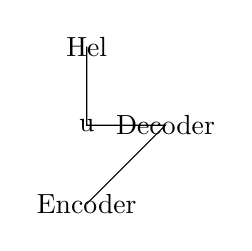
\begin{tikzpicture}

	\def\c{red!10!green!10!blue!80}

	%\node [circle, fill=gray] (decoder) at (0,0) {};
	%\node [rectangle, above=20, right=10, fill=\c] (encoder) at (decoder) {hello};
	%\node [rectangle, fill=gray] (output) at (encoder) ++(1,0) {};

	\draw
		(0,0) node (A) {Encoder} --
		+(1,1) node (B) {Decoder} --
		++(0,1) node (B) {u} --
		++(0,1) node (C) {Hel};

	%\draw[help lines, step=0.5] (0,0) grid (2,4);
	%\draw (decoder) to[out=180, in=0] (encoder);
\end{tikzpicture}

\caption{}
\figsource{}
\label{}

\end{figure}



\subsection{Usage}
This work uses a simplified implementation of the Generative Query Network.

In this work a network the architecture of GQN differs from the implementation used in the original paper. Here I use simple dense models for encoder and decoder that don't use random latent variables. This circumvents the necessity of having to use the evidence lower bound as an optimization target.

This however prevents the network from taking into account the inputs given during inference to the same extent as in the original experiments described in the paper. The only meaningful considerations of the inputs of the network were found to be the coloring of the sky, floor and walls (when the latter view have the same color). In the original implementation the network can correctly infer more properties like object position, rotation and texture.

Because interesting use cases where found, that do not depend on this property of the GQN network no more effort was put into recreating the ability of the network to model different scenes.
